

% (sources will be added later)

% ( foundatios to the thesis this chapter is.... state what it is and its importance should cover all the chapter)
This chapter provides the foundational concepts and underlying principles of the research.
It delves into the foundational concepts of Computer Vision and Deep Learning, illuminating on specific algorithms
and their underlying principles. The importance of reproducibility in scientific research is highlighted, with a particular focus 
on the challenges introduced by randomness in deep learning. This section further dissects the sources of this randomness, 
emphasizing the role of floating-point arithmetic. To provide a practical context, an overview  of
the various methods and tools utilized in this research, including optimizers, schedulers, and tracking tools, is presented. 
The aim is to ensure that readers, even those with a peripheral association with the field, can grasp the technical concepts and 
terminologies used throughout the thesis.
\section{Deep Learning}

\subsection{History of Rise of AI and Deep Learning}


Artificial Intelligence (AI) and its specialized branch, Deep Learning, trace their roots back to 1943 when Walter Pitts and Warren McCulloch~\cite{mcculloch1943logical} introduced a model based on human neural networks. This foundation led to the introduction of backpropagation in the 1960s and the development of convolutional neural networks by Kunihiko Fukushima~\cite{fukushima1980neocognitron} in the 1970s. Despite experiencing two significant setbacks known as the AI winters in the 1970s and late 1980s, the field saw major breakthroughs with the advent of support vector machines~\cite{cortes1995support} and LSTM networks~\cite{Hochreiter1995LONGST}.\\


The 21st century marked a transformative era for Deep Learning. Challenges like the Vanishing Gradient Problem~\cite{279181} were addressed, and the launch of the ImageNet database~\cite{5206848} in 2009 catalyzed advancements in image recognition. By 2011, with faster GPUs, architectures like AlexNet~\cite{NIPS2012_c399862d} emerged, outperforming traditional methods in international competitions. The pursuit of unsupervised learning was exemplified by Google Brain's Cat Experiment in 2012~\cite{google2023brain}. The inception of the Generative Adversarial Neural Network (GAN)~\cite{goodfellow2014generative} in 2014 further showcased the potential and versatility of deep neural networks.These milestones are summarized in chronological order in Table~\ref{tab:milestones}.\\

The resurgence and widespread adoption of Deep Learning in the 21st century can be attributed to two key factors: Big Data and computational power. The explosion of Big Data came first, announced by the onset of the digital age and the accumulation of massive datasets. This was closely followed by advancements in computational power, particularly the capabilities of GPUs, which made it feasible to process these large datasets. The synergy of vast amounts of data and the capability to process it efficiently enabled the Deep Learning algorithms, which had been conceptualized decades ago, to finally deliver on their potential and gain immense popularity.\\

\begin{table}[htbp]
    \centering
    \caption{Milestones in the Evolution of Neural Networks and AI}
    \label{tab:milestones}
    \begin{tabular}{|l|p{\textwidth - 3cm}|}
        \hline
        \textbf{Year} & \textbf{Milestone} \\
        \hline
        1943 & Introduction of Neural Network Model by Pitts \& McCulloch \\
        \hline
        1960s & Development of Backpropagation \\
        \hline
        1970s & First AI Winter \& Introduction of Convolutional Neural Networks by Fukushima \\
        \hline
        1985-1990s & Second AI Winter \& Advent of Support Vector Machines and LSTM \\
        \hline
        Early 2000s & Onset of the Big Data Era \\
        \hline
        2009 & Launch of ImageNet \\
        \hline
        Late 2000s & Exponential growth in GPU capabilities \\
        \hline
        2011 & Emergence of AlexNet \\
        \hline
        2012 & Google Brain's Cat Experiment \\
        \hline
        2014 & Introduction of Generative Adversarial Networks (GANs) by Ian Goodfellow \\
        \hline
    \end{tabular}
\end{table}


\subsection{Advancements and Significance of Deep Learning in the Modern Technological Landscape}
Deep learning has firmly established itself as one of the top technological advancements of the modern era. 
This technology, by emulating the structure and functionalities of the human brain through complex artificial neural networks, enables machines to 
learn and make independent decisions by processing vast data troves.\\

As illustrated in Figure~\ref{fig:trad_and_deep}, the primary distinction between traditional machine learning and deep learning lies in the approach to feature extraction. Traditional machine learning relies heavily on manual feature extraction, which necessitates human intervention to identify the most relevant features in the data before it can be used in a model. This manual step is not only labor-intensive but can also introduce biases and overlook potentially significant features, thereby constraining the model's effectiveness and scalability.\\

On the other hand, deep learning automates the feature extraction process, leveraging multi-layered neural networks to discern and extract essential features from the input data autonomously. This automation significantly accelerates the model training process and enhances the model's ability to generalize across various tasks. Moreover, as the model is exposed to more data, it can continually learn and improve, identifying intricate patterns and relationships that might elude a human analyst. The benefits of automatic feature extraction in deep learning, as depicted in Figure~\ref{fig:sources}, underscore its superiority over traditional machine learning in handling complex, high-dimensional data, and fueling innovation across a myriad of domains including image and speech recognition, medical diagnosis, and natural language processing.
\\

\begin{figure}[htbp]
    \centerline{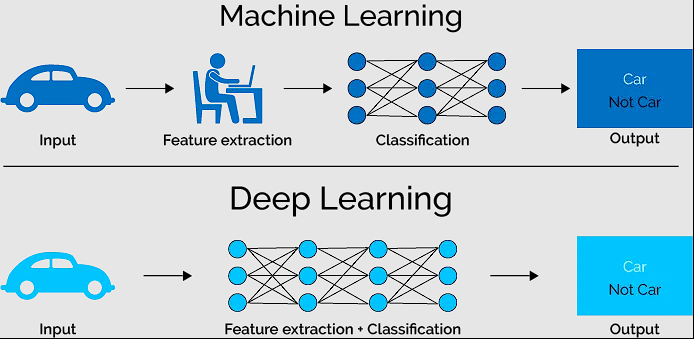
\includegraphics[scale=.75]{figures/traditional_vs_deeplearning.png}}
    \caption{Side-by-side comparison of traditional machine learning (with manual feature extraction) and deep learning (automatic feature extraction)~\cite{mahapatra2018deep}.}
    \label{fig:trad_and_deep}
    \end{figure}


The advancement of automation has only bolstered Deep Learning's relevance. 
In diverse applications, from robotic processes to customer service automation 
and even the intricate algorithms guiding self-driving vehicles, deep learning 
acts as the backbone. It provides these systems the tools to comprehend their 
environment and subsequently make informed decisions. This integration ensures 
not only unprecedented speed and efficiency but also a level of reliability and 
precision often surpassing human-driven processes.\\

Another frontier that deep learning is significantly influencing is Industry 4.0. 
This term, synonymous with the Fourth Industrial Revolution, marks the ongoing 
transformation characterized by heightened automation and data exchange in manufacturing 
technologies. It encompasses innovations like cyber-physical systems, the ever-expanding 
Internet of Things (IoT), cloud and cognitive computing. Within this ecosystem, deep learning 
emerges as a game-changer. Imagine a manufacturing setup where sensors constantly relay data 
from equipment. Deep learning models, acting on this data, can preemptively detect when a 
component might fail, ensuring timely maintenance, drastically reducing downtime, and 
invariably enhancing production efficiency.\\

To encapsulate, the significance of deep learning in our evolving technological 
landscape is huge. Whether it’s in the seemingly mundane, like fine-tuning song or movie recommendations, or in the deeply impactful, such as diagnosing ailments from medical images or forecasting calamities, deep learning prevails. 
As the world becomes increasingly data-centric, the unparalleled processing and analytical 
capabilities of deep learning models ensure that they remain not just relevant, but 
indispensable. In many ways, deep learning is not merely a trend within artificial 
intelligence; it represents an bold stride towards devising machines that think and 
learn akin to humans, yet operate on scales unfathomable to human cognition.\\

\subsection{Deep Learning Essentials}

Deep learning has become a driving force behind various state-of-the-art applications in numerous domains. The following core concepts elucidate the foundational pillars of deep learning, providing insights into its inner workings and methodologies.

\subsubsection*{Neural Networks}

\begin{figure}[htbp]
    \centering
    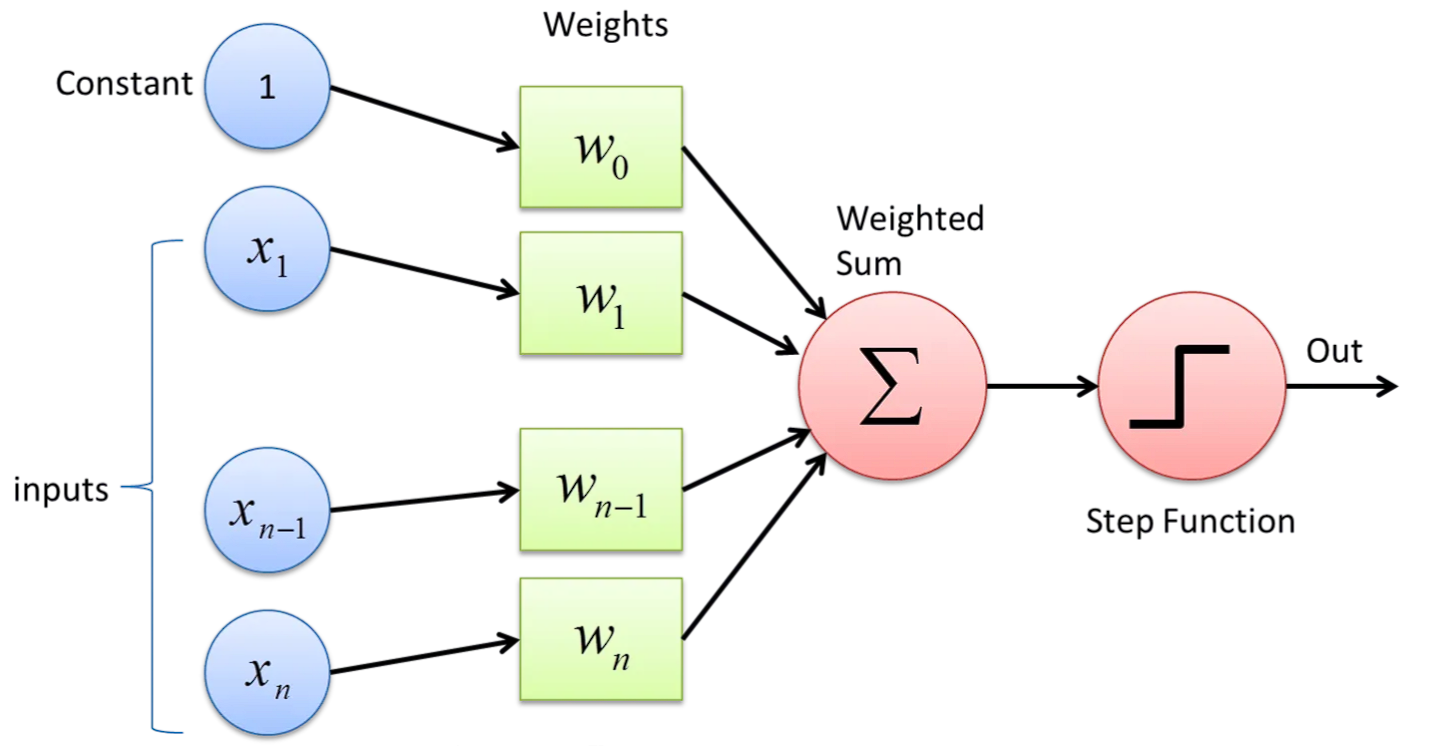
\includegraphics[width=\textwidth]{figures/perceptron.png}
    \caption{A perceptron, the basic building block of neural networks.~\cite{sharma2017perceptron} }
    \label{fig:perceptron}
\end{figure}

Neural networks are the foundational building blocks of deep learning. They are inspired by the structure and functioning of the human brain's interconnected neurons. The concept of neural networks has gained immense popularity due to their ability to learn complex patterns and representations from data. By simulating the interconnectedness of neurons, neural networks can capture hierarchical features in data, making them suitable for tasks such as image recognition, natural language processing, and more. The layers in a neural network (input, hidden, and output) allow for the extraction of progressively abstract features from the input data, enabling the model to make accurate predictions.

The fundamental unit of a neural network is a perceptron, as illustrated in Figure~\ref{fig:perceptron}. Proposed by Frank Rosenblatt in 1957, the perceptron marked the inception of automated feature extraction, a cornerstone of deep learning's superiority over traditional machine learning. Rosenblatt's seminal work, titled "The Perceptron, a Perceiving and Recognizing Automaton," showcased the initial steps towards automating the identification of essential features in data, a concept that is deeply ingrained in today's deep learning models~\cite{rosenblatt1957perceptron}.

\subsubsection*{General Structure of an Artificial Neural Network}
An Artificial Neural Network (ANN) comprises three main types of layers: the input layer, hidden layers, and the output layer. 

\begin{itemize}
    \item \textbf{Input Layer:} The input layer consists of neurons that receive the input data and pass it on to the network. Each neuron in this layer corresponds to one feature in the input data.
    \item \textbf{Hidden Layers:} The hidden layers contain neurons that perform computations and transfer information from the input layer to the output layer. The complexity of the neural network increases with the number of hidden layers and the number of neurons in each hidden layer.
    \item \textbf{Output Layer:} The output layer contains neurons that provide the final output of the network. The type of problem (e.g., binary classification, multi-class classification, regression) dictates the number of neurons in the output layer and the activation function used.
\end{itemize}

Each neuron in a layer is connected to all neurons in the previous and subsequent layers, and these connections have associated weights. The weights (\(w\)) and biases (\(b\)) are parameters that are learned from the data during training. They are crucial for the network's ability to make accurate predictions. The weights control the strength of the connection between two neurons, and the biases allow the neurons to have some flexibility in activation. During the training process, the weights and biases are adjusted to minimize the difference between the predicted output and the actual target values, making the model more accurate over time. This process is driven by the backpropagation algorithm, which computes gradients of the loss function with respect to the weights and biases. The activation function within each neuron introduces non-linearity, enabling the network to learn complex patterns. The loss function quantifies the discrepancy between the network's predictions and the actual data, guiding the optimizer in adjusting the weights and biases to minimize this loss.

The output \( y \) of a neuron is given by the equation:
\[
y = f(\mathbf{w} \cdot \mathbf{x} + b)
\]
where \( \mathbf{w} \) is the vector of weights, \( \mathbf{x} \) is the vector of inputs, \( b \) is the bias, and \( f \) is the activation function. A graphical illustration of the process within a neuron is depicted in Figure~\ref{fig:neuron_math}, showing the linear combination of weights and inputs, the addition of the bias, and the application of the activation function to produce the output.

\begin{figure}[htbp]
    \centering
    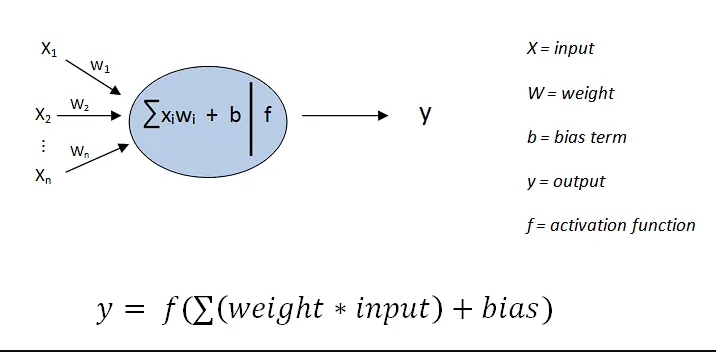
\includegraphics[width=\textwidth]{figures/weights_and_biases.png}
    \caption{Graphical representation of a neuron showing the weights, inputs, bias, and activation function.~\cite{yildirim2020activation}}
    \label{fig:neuron_math}
\end{figure}

\subsubsection*{Activation Functions}

Activation functions introduce non-linearity to the neural network, allowing it to approximate and learn complex relationships in data. Without activation functions, neural networks would only be capable of representing linear transformations, severely limiting their expressive power. ReLU, Sigmoid, and Tanh are commonly used activation functions, each with its unique properties. ReLU addresses the vanishing gradient problem, Sigmoid maps inputs to a sigmoid-shaped range suitable for binary classification, and Tanh is often used in hidden layers to map inputs to a range between -1 and 1. The mathematical expressions for these activation functions and in Figure \ref{fig:activation_functions} a graph of these functions are presented below.

\begin{itemize}
    \item \textbf{ReLU (Rectified Linear Unit):} 
    \[ f(x) = \max(0, x) \]
    
    \item \textbf{Sigmoid:} 
    \[ f(x) = \frac{1}{1 + e^{-x}} \]
    
    \item \textbf{Tanh:} 
    \[ f(x) = \tanh(x) = \frac{2}{1 + e^{-2x}} - 1 \]
\end{itemize}

\begin{figure}[h!]
\centering
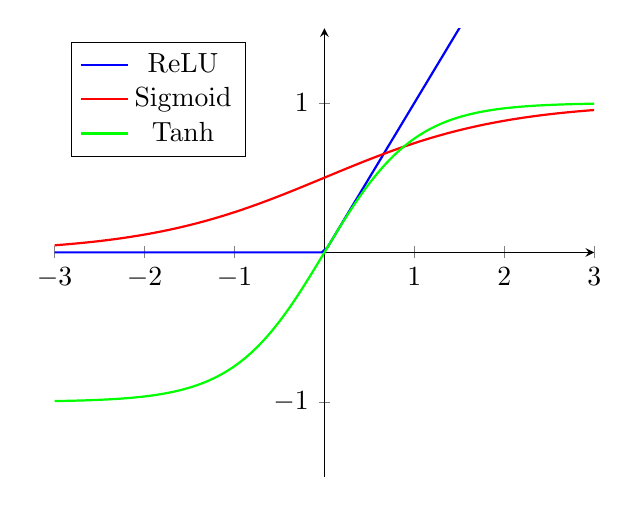
\begin{tikzpicture}
\begin{axis}[
  axis lines=center,
  domain=-3:3,
  ymax=1.5,
  ymin=-1.5,
  samples=100,
  legend pos=north west
]
\addplot[blue, thick] {max(0, x)}; 
\addplot[red, thick] {1/(1 + exp(-x))}; 
\addplot[green, thick] {(2/(1 + exp(-2*x))) - 1};
\legend{ReLU, Sigmoid, Tanh}
\end{axis}
\end{tikzpicture}
\caption{Visualization of Activation Functions}
\label{fig:activation_functions}
\end{figure}


\subsubsection*{Loss Functions}

Loss functions quantify the difference between predicted and true values, providing a measure of how well the model is performing. They serve as the basis for optimization, helping the model adjust its parameters to minimize the discrepancy between predictions and ground truth. Different loss functions are used for different tasks; Mean Squared Error (MSE) is well-suited for regression tasks, while Cross-Entropy is commonly used for classification tasks. The choice of the appropriate loss function depends on the nature of the problem the neural network is tackling.

\begin{itemize}
    \item \textbf{Mean Squared Error (MSE)} for regression tasks:
    \[ L(y, \hat{y}) = \frac{1}{n} \sum_{i=1}^{n} (y_i - \hat{y}_i)^2 \]

    MSE is used for regression tasks where we predict continuous values. It's chosen because it penalizes larger errors more, it's differentiable for efficient optimization, and its convex nature aids in finding optimal solutions.
    
    \item \textbf{Cross-Entropy} for classification:
    \[ L(y, \hat{y}) = -\sum_{i} y_i \log(\hat{y}_i) \]

    Cross-Entropy is for classification tasks. It's based on probabilities, making it suitable for class probabilities interpretation. Its logarithmic nature amplifies differences between predicted and true class probabilities, aiding optimization. Also, its gradient doesn't saturate, ensuring continuous learning.

\end{itemize}


% \todo[inline]{Visualization: You can insert specific diagrams or visualizations for Loss Functions}


\subsubsection*{Optimizers}

Optimizers play a crucial role in training neural networks by adjusting the model's parameters to minimize the loss function. Gradient Descent and its variants, such as Stochastic Gradient Descent (SGD), SGD with Momentum, and Adam, are pivotal in this endeavor. These optimizers iteratively modify the model parameters, aiming to find the minima of the loss function, which in turn enhances the model's performance.

\begin{itemize}
    \item \textbf{Gradient Descent (GD):} The algorithm aims to find the minimum of a function \( F \) by iteratively moving in the direction of steepest descent, as defined by the negative of the gradient \( \nabla F \) at the current point \( \mathbf{x}_n \). The update rule is given by 
    \[ \mathbf {x}_{n+1} = \mathbf {x}_n - \gamma_n \nabla F(\mathbf {x}_n),\ n\geq 0 \]
    where \( \gamma_n \) is the learning rate at iteration \( n \).

    \item \textbf{Stochastic Gradient Descent (SGD):} Unlike GD, SGD approximates the gradient using a single training example, which can lead to faster convergence. The update for each parameter \( w \) is 
    \[ w := w - \eta \nabla Q_i(w) \]
    where \( \eta \) is the learning rate.

    \item \textbf{SGD with Momentum:} This variant accelerates SGD by adding a momentum term, which serves to dampen oscillations and speed up convergence. The update rule is:
    \[ v_t = \mu v_{t-1} - \eta \nabla Q_i(w) \]
    \[ w := w + v_t \]
    where \( \mu \) is the momentum term. (See \textit{On the importance of initialization and momentum in deep learning} by Sutskever et al.,~\cite{sutskever2013importance} for more details.).

    \item \textbf{Adam:} The update rule for the parameters \( w \) in Adam is defined as 
    \[ w_{t} = w(t-1) - \alpha \cdot \left( \frac{\hat{m_t}}{\sqrt{\hat{v_t}} + \epsilon} \right), \]
    where \( w_t \) and \( w(t-1) \) are the parameter vectors at time \( t \) and \( t-1 \) respectively, \( \alpha \) is the learning rate, \( \hat{m_t} \) and \( \hat{v_t} \) are bias-corrected estimates of the first and second moment, and \( \epsilon \) is a small constant to prevent division by zero.
\end{itemize}




\subsubsection*{Backpropagation}

Backpropagation is a fundamental algorithm for training neural networks. It is vital because it enables neural networks to learn from data by adjusting their weights and biases. The process involves calculating the gradients of the loss function with respect to each parameter using the chain rule from calculus. These gradients guide the optimization algorithm in adjusting the model's parameters to minimize the prediction error. To visually represent how backpropagation operates within a neural network, we present Figure \ref{fig:backrop} below. Backpropagation is crucial for enabling neural networks to learn complex relationships in data, as it iteratively fine-tunes the model's parameters based on the feedback provided by the gradients.

\begin{figure}[htbp]
    \centerline{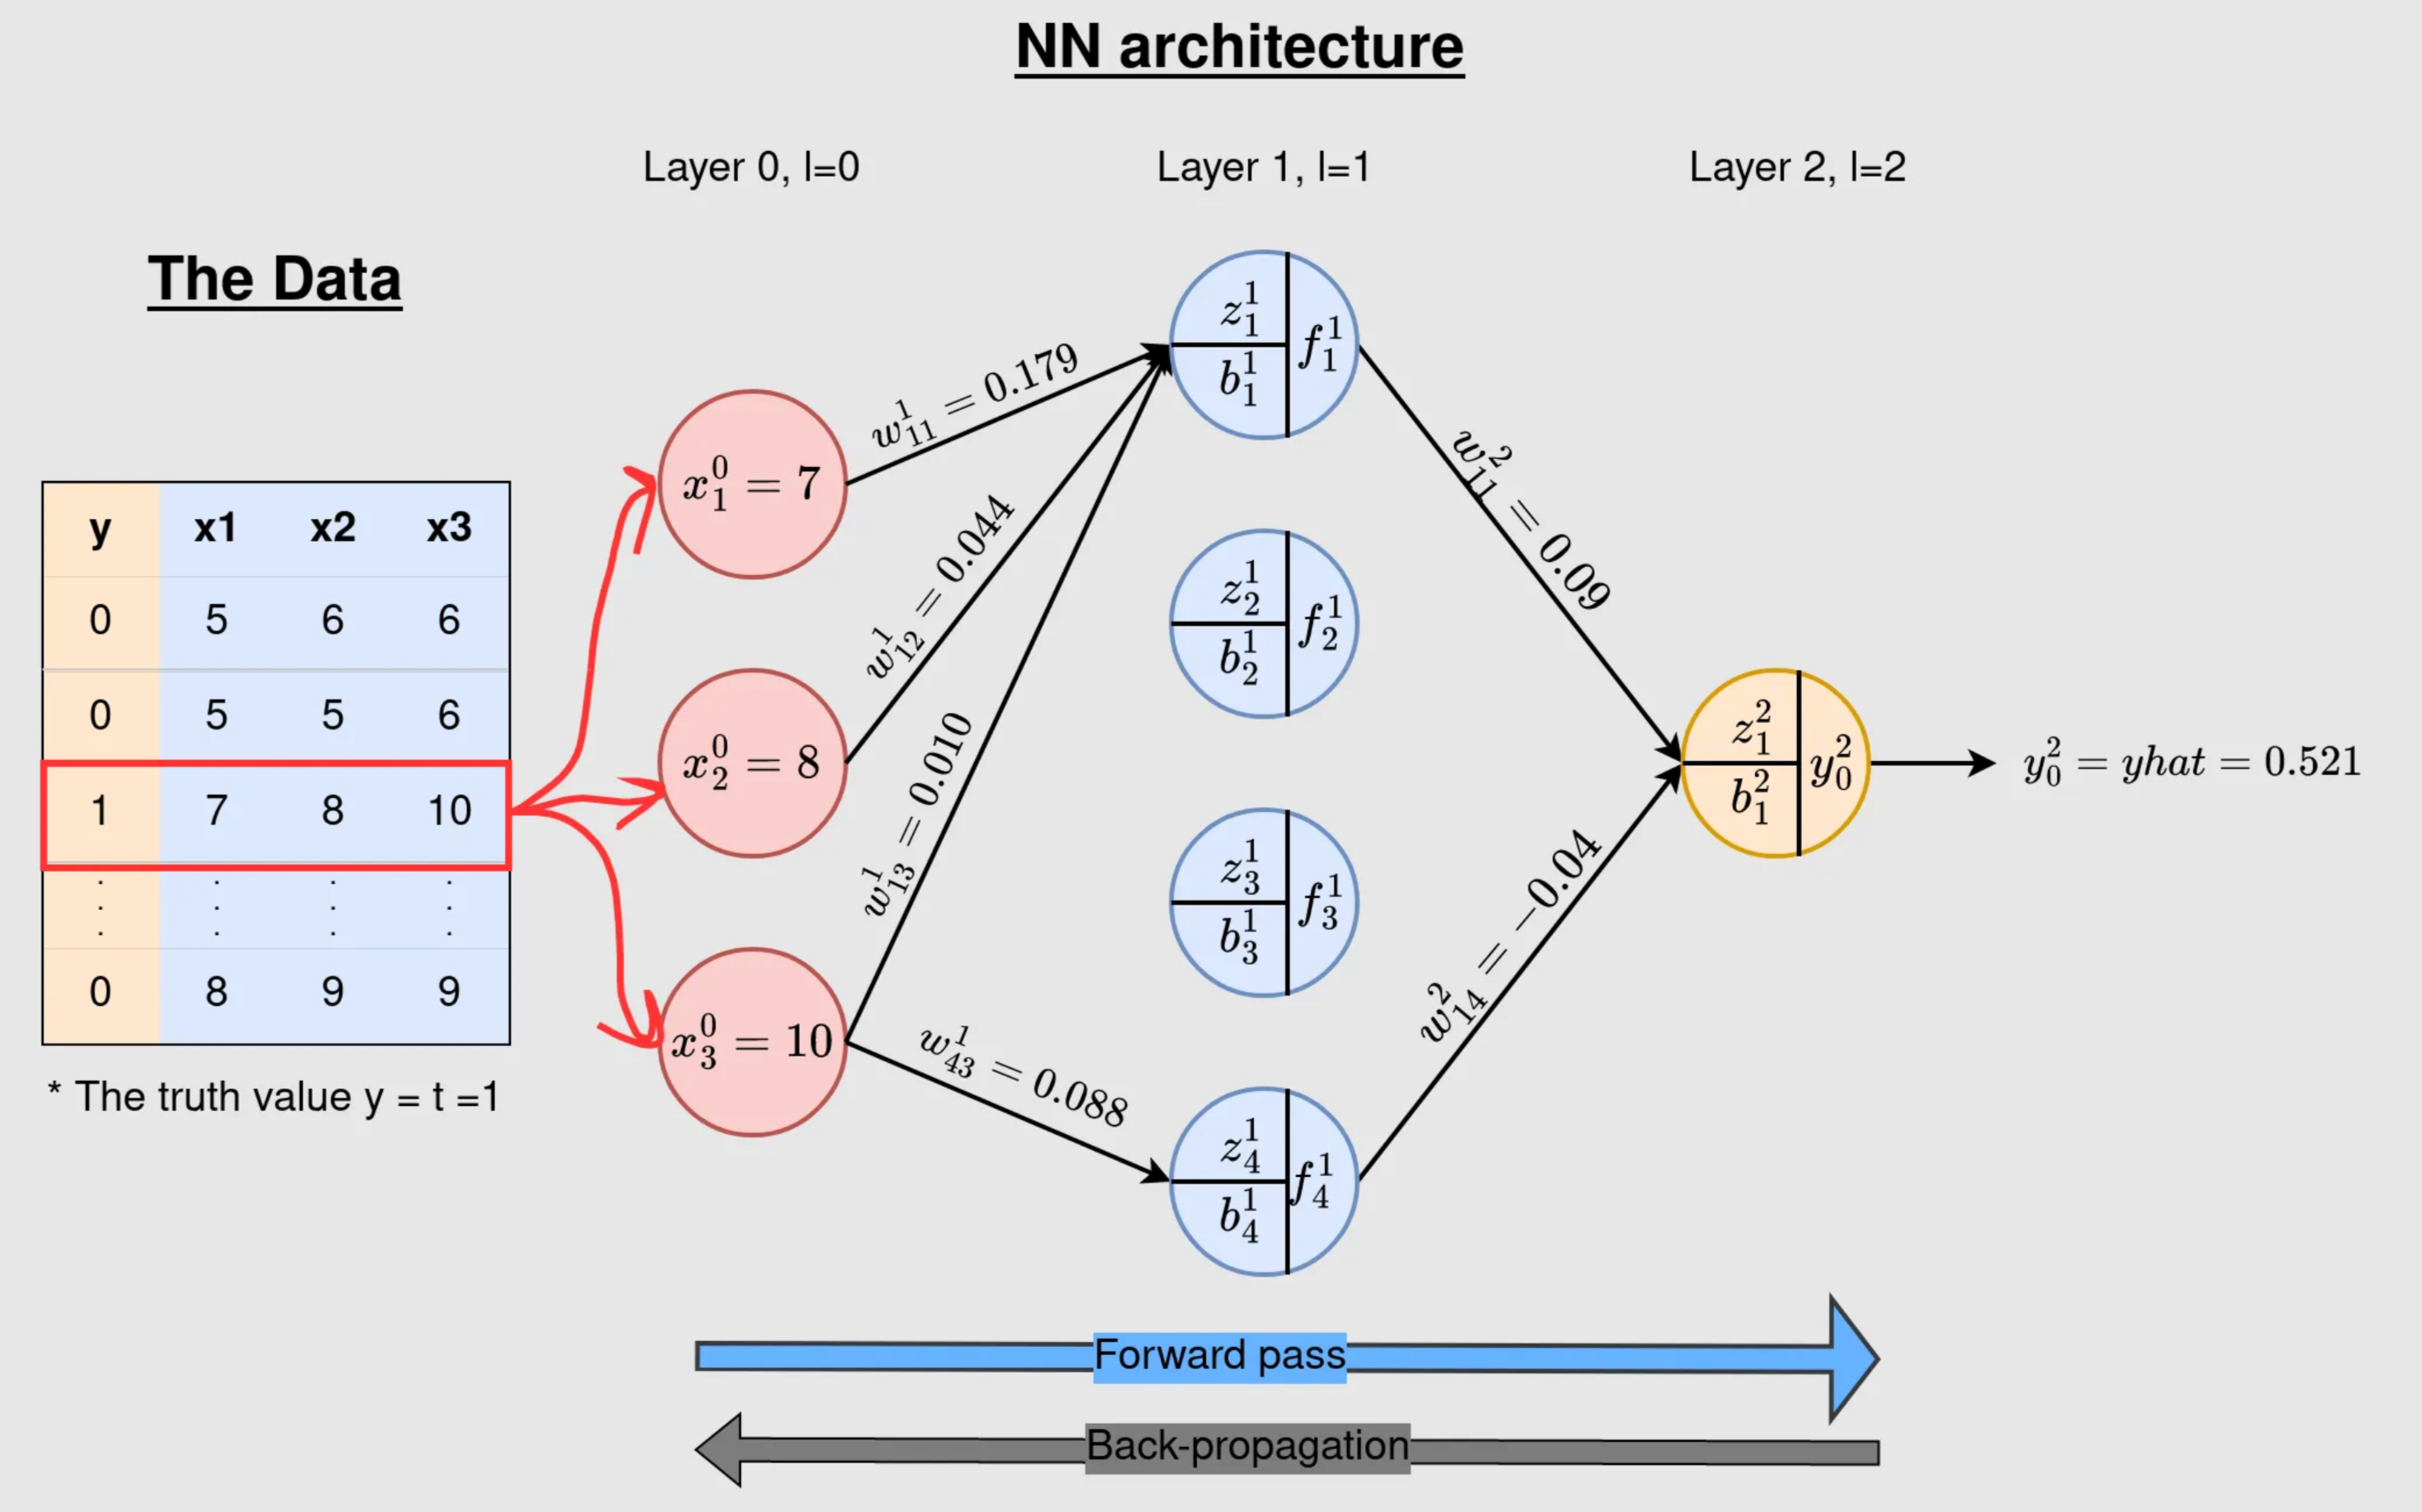
\includegraphics[scale=.29]{figures/backpropagation.png}}
    \caption{Example basic Neural Network Architecture~\cite{koech2022backpropagation} }
    \label{fig:backrop}
    \end{figure}

Following, with reference to Figure \ref{fig:backrop}, we try to explain the simple weight optimization process with backpropagation:\\

\textbf{1. Activation Function (Sigmoid):}
The sigmoid function, \( \sigma(z) \), and its derivative are given by:
\begin{align*}
\sigma(z) &= \frac{1}{1 + e^{-z}} \\
\sigma'(z) &= \sigma(z)(1 - \sigma(z))
\end{align*}

\textbf{2. Loss Function (Cross-Entropy Loss):}
For binary classification tasks, the cross-entropy loss for a predicted output \( y \) and true target \( t \) is:
\[
L(y, t) = -t \log(y) - (1 - t) \log(1 - y)
\]

\textbf{3. Gradient of the Loss:}
The gradient of the cross-entropy loss with respect to the output \( y \) is:
\[
\frac{\partial L}{\partial y} = \frac{y - t}{y(1 - y)}
\]

\textbf{4. Backpropagation:}
For a single-layer neural network, the gradient of the loss \( L \) with respect to the weight \( w \) is:
\begin{align*}
\frac{\partial L}{\partial w} &= \frac{\partial L}{\partial y} \times \frac{\partial y}{\partial z} \times \frac{\partial z}{\partial w} \\
\frac{\partial L}{\partial w} &= \frac{y - t}{y(1 - y)} \times \sigma(z)(1 - \sigma(z)) \times x
\end{align*}
where \( z = w \cdot x + b \). \\

\textbf{5. Weight Update using SGD:}
The weight is updated as:
\[
w_{\text{new}} = w_{\text{old}} - \alpha \times \frac{\partial L}{\partial w}
\]
Where \( \alpha \) is the learning rate.
\subsubsection*{Batch Normalization}

Batch Normalization is a technique that improves the training stability and convergence speed of neural networks. It normalizes the intermediate feature representations within a neural network batch-wise. This process helps mitigate the vanishing and exploding gradient problems, enabling smoother and faster convergence during training. Batch Normalization also acts as a regularizer, reducing the need for other regularization techniques like dropout.
\[ \hat{x} = \frac{x - \mu}{\sqrt{\sigma^2 + \epsilon}} \]
Where \( \mu \) is the mean and \( \sigma^2 \) is the variance.

\subsubsection*{Transfer Learning}

Transfer Learning leverages knowledge gained from one task or dataset to improve performance on another related task or dataset. This approach is incredibly useful when labeled data is scarce for the target task. Pre-trained models, especially those trained on massive datasets like ImageNet, provide valuable initializations for the model's parameters. Fine-tuning a pre-trained model on a specific task allows the model to learn task-specific features while retaining the general knowledge it gained from the pre-training.\\

However, there can be disadvantages such as negative transfer where the pre-training may misguide the learning on the target task, or overfitting if the target task's dataset is too small.
\begin{itemize}
    \item \textbf{Learning Rate:} This is a crucial hyperparameter that determines the step size taken during each iteration while moving towards a minimum in the loss function. A smaller learning rate might take longer to converge, as it involves tiny steps, but a larger one risks overshooting the optimal point. Properly tuning the learning rate ensures that the model learns efficiently without getting stuck or overshooting.
    
    \item \textbf{Batch Size:} It refers to the number of training samples used in one iteration to update a model's weights. A smaller batch size might lead to more frequent updates, making the model converge faster but possibly with less stability. On the other hand, a larger batch size provides a more general estimate of the gradient, but it requires more memory and might slow down the training.
    
    \item \textbf{Network Architecture:} This refers to the design and structure of the neural network, including the number of layers, the number of units in each layer, and the connections between them. The architecture defines the complexity and capacity of the model. Selecting the right architecture is crucial as it can influence the model's ability to capture intricate patterns in the data.
\end{itemize}

Efficiently tuning these hyperparameters is a challenge but doing so can lead to faster convergence and better model generalization. Techniques like grid search, random search, and Bayesian optimization help navigate the high-dimensional space of hyperparameters to find optimal combinations.~\cite{Claesen2015HyperparameterSI}

\subsubsection*{Performance Metrics}

Performance Metrics quantify how well a model is performing on specific tasks. They provide insights into the model's strengths and weaknesses. 

For classification tasks:

\begin{itemize}
    \item \textbf{Precision:} It is the ratio of correctly predicted positive observations to the total predicted positives.
    \[ \text{Precision} = \frac{\text{True Positives}}{\text{True Positives} + \text{False Positives}} \]

    \item \textbf{Recall (Sensitivity):} It is the ratio of correctly predicted positive observations to all the actual positives.
    \[ \text{Recall} = \frac{\text{True Positives}}{\text{True Positives} + \text{False Negatives}} \]

    \item \textbf{F1-Score:} It is the weighted average of Precision and Recall. It tries to find the balance between precision and recall.
    \[ \text{F1-Score} = 2 \times \frac{\text{Precision} \times \text{Recall}}{\text{Precision} + \text{Recall}} \]

    \item \textbf{ROC (Receiver Operating Characteristics) Curve:} The ROC curve is a graphical representation that illustrates the performance of a binary classifier system as its discrimination threshold is varied. It plots the True Positive Rate (TPR) against the False Positive Rate (FPR) at various threshold settings. The curve starts at the origin (0,0) and ends at (1,1). The diagonal line from (0,0) to (1,1) represents a random classifier, and a good classifier aims to stay as far away from this line as possible (towards the top-left corner).

    \item \textbf{AUC (Area Under The Curve):} It measures the entire two-dimensional area underneath the ROC curve (from (0,0) to (1,1)). AUC represents the degree or measure of separability, indicating how much the model distinguishes between the positive and negative classes.
\end{itemize}

For regression tasks, Mean Absolute Error (MAE) and Mean Squared Error (MSE) measure the deviation between predicted and true values, giving a clear picture of the prediction quality.

\begin{itemize}
    \item \textbf{Mean Absolute Error (MAE):}
    \[ \text{MAE} = \frac{1}{n} \sum_{i=1}^{n} |y_i - \hat{y}_i| \]
    Where:
    - \( n \) is the total number of data points or observations.
    - \( y_i \) is the actual value of the \( i^{th} \) observation.
    - \( \hat{y}_i \) is the predicted value of the \( i^{th} \) observation.
    - \( |y_i - \hat{y}_i| \) represents the absolute difference between the actual and predicted value for the \( i^{th} \) observation.

    \item \textbf{Mean Squared Error (MSE):}
    \[ \text{MSE} = \frac{1}{n} \sum_{i=1}^{n} (y_i - \hat{y}_i)^2 \]
    Where:
    - \( (y_i - \hat{y}_i)^2 \) represents the squared difference between the actual and predicted value for the \( i^{th} \) observation.
\end{itemize}
\subsubsection*{Data Augmentation}

Data Augmentation is essential for training robust and generalized models, particularly in domains like computer vision. By applying domain-specific transformations to the training data, the model becomes less sensitive to variations in the input data, such as rotation, scaling, and cropping. This technique effectively increases the diversity of the training dataset, helping the model learn more representative features and improving its ability to handle real-world data. For a comprehensive understanding and deeper insights into data augmentation techniques, we refer the reader to the seminal work of Shorten et al.~\cite{Shorten2019ASO}.
\subsubsection*{Learning Rate Schedulers}

Learning rate schedulers are algorithms or methods that adjust the learning rate during training based on the number of epochs, iterations, or other criteria. The learning rate is a crucial hyperparameter in training deep neural networks. If set too high, the training might diverge; if set too low, the training might be too slow or get stuck in local minima. By dynamically adjusting the learning rate, schedulers aim to combine the benefits of both high and low learning rates, leading to faster convergence and better generalization.

Here are some popular learning rate schedulers:

\begin{enumerate}
    \item \textbf{Step Decay}: Reduces the learning rate by a factor after a specified number of epochs.
    \item \textbf{Exponential Decay}: Decreases the learning rate at each epoch or iteration exponentially.
    \item \textbf{Cosine Annealing}: Adjusts the learning rate according to a cosine function.
    \item \textbf{ReduceLROnPlateau}: Reduces the learning rate when a metric has stopped improving.
    \item \textbf{Cyclic Learning Rates}: Allows the learning rate to cyclically vary between two bounds.
\end{enumerate}

We focus on the exponential LR and Cosine Annealing LR schedulers.\\

The formula for exponential decay is:

\begin{equation}
\text{lr}(t) = \text{lr}_\text{initial} \times \text{factor}^t
\end{equation}

Where:
\begin{itemize}
    \item $\text{lr}_\text{initial} = 0.001$
    \item $\text{factor} = 0.5$
\end{itemize}

\begin{figure}[h]
    \centering
    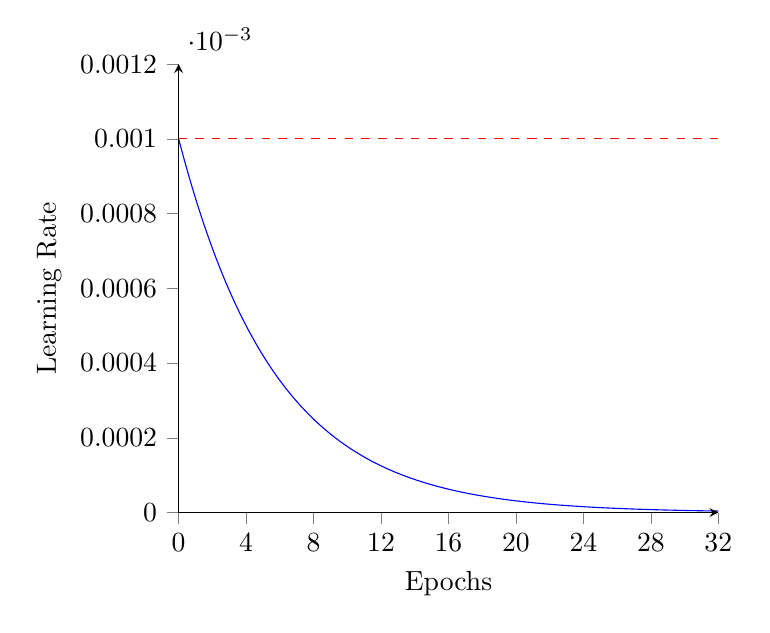
\begin{tikzpicture}
    \begin{axis}[
        xlabel=Epochs,
        ylabel=Learning Rate,
        domain=0:32,
        samples=100,
        axis lines=left,
        xmin=0, xmax=32,
        ymin=0, ymax=0.0012,
        xtick={0,4,8,12,16,20,24,28,32},
        ytick={0,0.0002,0.0004,0.0006,0.0008,0.001,0.0012},
        xticklabels={0,4,8,12,16,20,24,28,32},
        yticklabels={0,0.0002,0.0004,0.0006,0.0008,0.001,0.0012},
        tick align=outside,
        axis on top,
        smooth
    ]
    \addplot [mark=none,color=blue] {0.001 * 0.5^(x / 4)};
    \addplot [mark=none,color=red,dashed] coordinates {(0,0.001) (32,0.001)};
    \end{axis}
    \end{tikzpicture}
    \caption{Exponential Learning Rate Schedule (Decay Factor = 0.5)}
\end{figure}

The formula for cosine annealing is:

\begin{equation}
\text{lr}(t) = \text{lr}_\text{min} + \frac{1}{2}(\text{lr}_\text{max} - \text{lr}_\text{min})(1 + \cos(\frac{\pi t}{T}))
\end{equation}

Where:
\begin{itemize}
    \item $\text{lr}_\text{min} = 0$ (usually)
    \item $\text{lr}_\text{max} = 0.001$
    \item $T = 32$
\end{itemize}

In the figure \ref{fig:exponential} we can see the graph cosine annealing learning rate schedule.

\begin{figure}[h!]
    \centering
    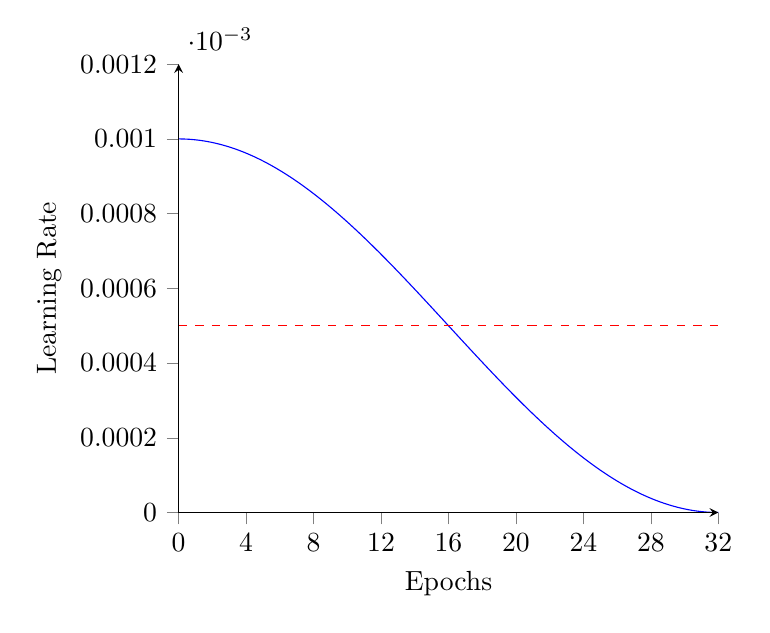
\begin{tikzpicture}
    \begin{axis}[
        xlabel=Epochs,
        ylabel=Learning Rate,
        domain=0:32,
        samples=100,
        axis lines=left,
        xmin=0, xmax=32,
        ymin=0, ymax=0.0012,
        xtick={0,4,8,12,16,20,24,28,32},
        ytick={0,0.0002,0.0004,0.0006,0.0008,0.001,0.0012},
        xticklabels={0,4,8,12,16,20,24,28,32},
        yticklabels={0,0.0002,0.0004,0.0006,0.0008,0.001,0.0012},
        tick align=outside,
        axis on top,
        smooth
    ]
    \addplot [mark=none,color=blue] {0.0005 * (1 + cos(180 * x / 32))};
    \addplot [mark=none,color=red,dashed] coordinates {(0,0.0005) (32,0.0005)};
    \end{axis}
    \end{tikzpicture}
    \caption{Cosine Annealing Learning Rate Schedule}
    \label{fig:exponential}
\end{figure}


\subsubsection*{Early Stopping}

Early Stopping is a regularization technique used to prevent overfitting. Training a model for too many epochs can lead to it memorizing the training data rather than generalizing to new data. Early Stopping monitors the validation performance and halts training when the validation loss starts to increase. This prevents the model from deteriorating on unseen data and helps achieve the best trade-off between training performance and generalization.
% You can insert a visualization here showing training vs validation loss and pointing out where early stopping would intervene.


\subsection{Overview of Deep Learning Algorithms}

Deep learning, over the years, has evolved to cater to diverse domains and challenges, leading to the development of several specialized algorithms. These algorithms emerged in response to specific challenges in data representation, computational efficiency, or domain-specific nuances. The diversity in algorithms is primarily a result of attempts to optimize performance across a myriad of tasks.\\

In chronological order, some of the influential deep learning architectures include Feedforward Neural Networks, Convolutional Neural Networks (CNNs), Recurrent Neural Networks (RNNs), Long Short-Term Memory (LSTM) networks, Gated Recurrent Units (GRUs), and Transformer Networks. A brief overview of these algorithms is presented in Table~\ref{tab:deep_learning_overview}.

\begin{table}[h]
\centering
\begin{tabularx}{\linewidth}{|l|X|}
\hline
\textbf{Algorithm} & \textbf{Description} \\
\hline
Feedforward Neural Networks & Early architectures designed for pattern recognition without any cycles or loops. \\
\hline
CNNs & Specialized for processing grid-like data, such as images, using convolutional layers. \\
\hline
RNNs & Designed for sequential data, containing loops to maintain information across sequences. \\
\hline
LSTM & An RNN variant addressing vanishing gradient issues and retaining long-term dependencies. \\
\hline
GRUs & Simplified version of LSTMs, offering similar capabilities with fewer parameters. \\
\hline
Transformer Networks & Attention-based models providing parallel processing capabilities and superior performance in sequence tasks. \\
\hline
\end{tabularx}
\caption{Brief overview of key deep learning algorithms.}
\label{tab:deep_learning_overview}
\end{table}




\subsubsection*{Convolutional Neural Networks}

Convolutional Neural Networks (CNNs), which began to emerge in the 1980s and gained significant popularity by the late 2000s, have brought transformative changes to the field of image processing. One of the pioneering CNNs, the Neocognitron, was introduced by Fukushima in 1980~\cite{fukushima1980neocognitron}. This was followed by LeNet-5, a work by LeCun et al. in 1998~\cite{lecun1995convolutional}. More recent advancements in CNN architectures include models like ConvNeXt~\cite{liu2022convnet} and EfficientNetV2~\cite{tan2021efficientnetv2}.\\ 

Distinct from traditional Feedforward Neural Networks (FNNs)---which process inputs through a series of interconnected layers without loops or cycles---CNNs incorporate convolutional layers. These layers utilize filters to scan an input for specific patterns. This convolutional process significantly reduces the number of parameters in the network, allowing the model to recognize local patterns in data more efficiently.

\begin{figure}[htbp]
    \centering
    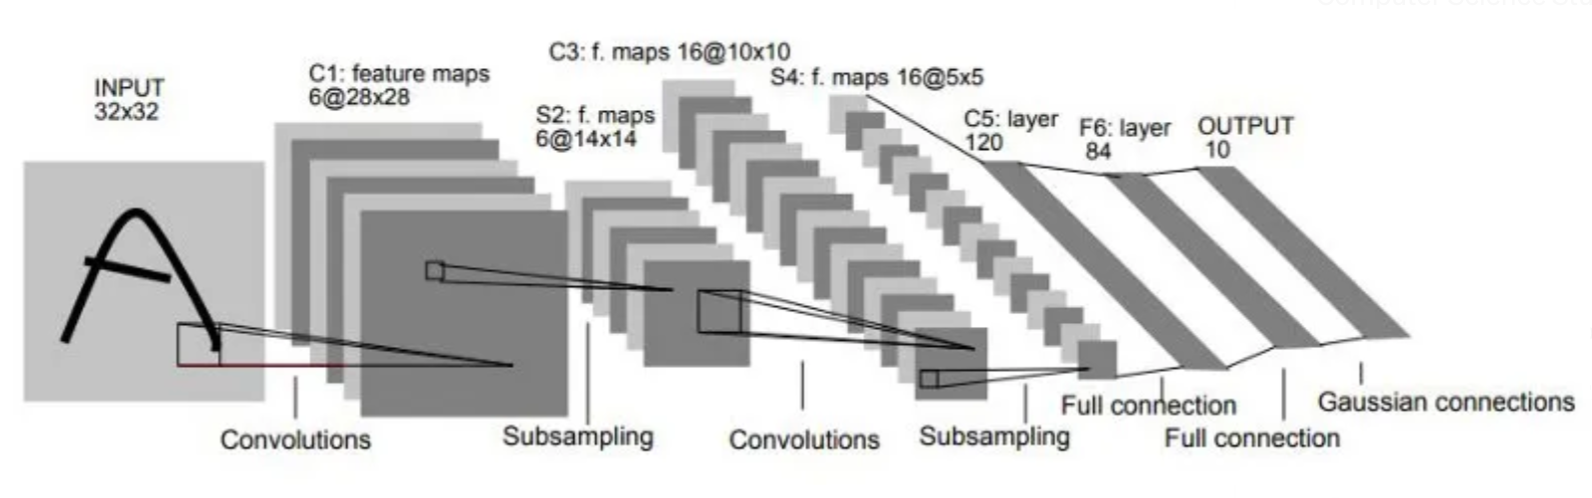
\includegraphics[scale=.5]{figures/lenet.png}
    \caption{Example structure of a CNN~\cite{lecun1995convolutional}. }
    \label{fig:lenet}
\end{figure}

Advantages of CNNs include Parameter Efficiency, which refers to the reduced parameters due to shared weights in convolutional layers; Translation Invariance, highlighting the ability of CNNs to recognize patterns regardless of their position in the input; and Hierarchical Feature Learning, where deep architectures extract layered features, moving from basic to more complex patterns.

% Visualization idea for CNN: A diagram showing how an image is passed through convolutional layers, pooling layers, and fully connected layers.

\subsubsection*{Transformer Networks}
Introduced in the "Attention Is All You Need" paper by Vaswani et al. in 2017~\cite{vaswani2023attention}, Transformers have since dominated various sequence-based tasks, especially in natural language processing. Instead of relying on recurrence, they use self-attention mechanisms to weigh the importance of different parts of the input data.\\

\textbf{Advantages of Transformer Networks:}
\begin{itemize}
    \item \textit{Parallel Processing:} Lack of recurrence allows simultaneous processing of sequence data, leading to speed gains.
    \item \textit{Long-Distance Dependencies:} Captures relationships in data regardless of the distance between elements.
    \item \textit{Scalability:} Easily scales to handle vast datasets and offers state-of-the-art results in many domains.
\end{itemize}

\textbf{Applications:}
\begin{itemize}
    \item Natural Language Processing tasks like translation, summarization, and question-answering.
    \item Time-series forecasting.
    \item Some computer vision tasks leveraging the Vision Transformer architecture.
\end{itemize}

% Visualization idea for Transformer: A diagram showcasing the self-attention mechanism, highlighting how different parts of an input sequence contribute to the output.
\subsection{Applications of Deep Learning}

Deep learning, an advanced subset of machine learning, has fostered a plethora of innovations across numerous domains due to its unparalleled proficiency in handling vast datasets and extracting intricate patterns. The applicability of deep learning transcends sectors, enabling tasks that were once considered the realm of science fiction. For a comprehensive understanding and deeper insights into deep learning and its applications, we refer the reader to the seminal work of Dong et al.~\cite{DONG2021100379}.\\

% \todo[inline]{Visualization: Montage or grid showcasing various applications of deep learning.}
\begin{itemize}
    \item \textbf{Computer Vision:} From basic image classification to advanced tasks like object detection, segmentation, and facial recognition, deep learning, particularly through Convolutional Neural Networks (CNNs), has redefined the boundaries of what machines can perceive. Autonomous vehicles, medical image analysis, and augmented reality are just a few sectors harnessing the power of deep learning-driven computer vision.
    
    \item \textbf{Natural Language Processing (NLP):} Transformer architectures, most notably the BERT and GPT series, have drastically improved machines' ability to understand and generate human language. This has led to improvements in machine translation, sentiment analysis, and chatbots.
    
    \item \textbf{Speech Recognition:} Voice assistants like Siri, Alexa, and Google Assistant are a testament to the prowess of deep learning in understanding and synthesizing human speech, making voice-activated systems more accurate and ubiquitous.
    
    \item \textbf{Healthcare:} From diagnosing diseases with medical imaging to predicting patient trajectories, deep learning is assisting medical professionals by providing tools that can spot symptoms and patterns often too subtle for the human eye.
    
    \item \textbf{Finance:} In the world of finance, algorithms can predict stock market fluctuations, detect fraudulent activities, and automate trading by leveraging deep learning models.
    
    \item \textbf{Entertainment:} Deep learning-driven recommendation systems, such as those employed by Netflix and Spotify, personalize content suggestions, enhancing user experience. Also, Generative Adversarial Networks (GANs) have been used for art creation, game design, and even music generation.
\end{itemize}

While each of these domains has been transformed by the introduction of deep learning, our primary focus will be on \textbf{Computer Vision}. In the subsequent sections, we will delve deep into its intricacies, methodologies, and advancements, painting a comprehensive picture of how machines `see' and `interpret' visual data.
\section{Computer Vision}

Computer Vision (CV) is an interdisciplinary field that seeks to enable machines to interpret and make decisions based on visual data. Drawing inspirations from human vision, pattern recognition, and computational intelligence, CV has emerged as one of the most significant application areas for deep learning. As \textit{Hubel and Wiesel} pointed out in their groundbreaking studies 
on the visual cortex~\cite{Hubel1962ReceptiveFB}, understanding vision is quintessential to understanding intelligence itself.

\begin{figure}[htbp]
    \centering
    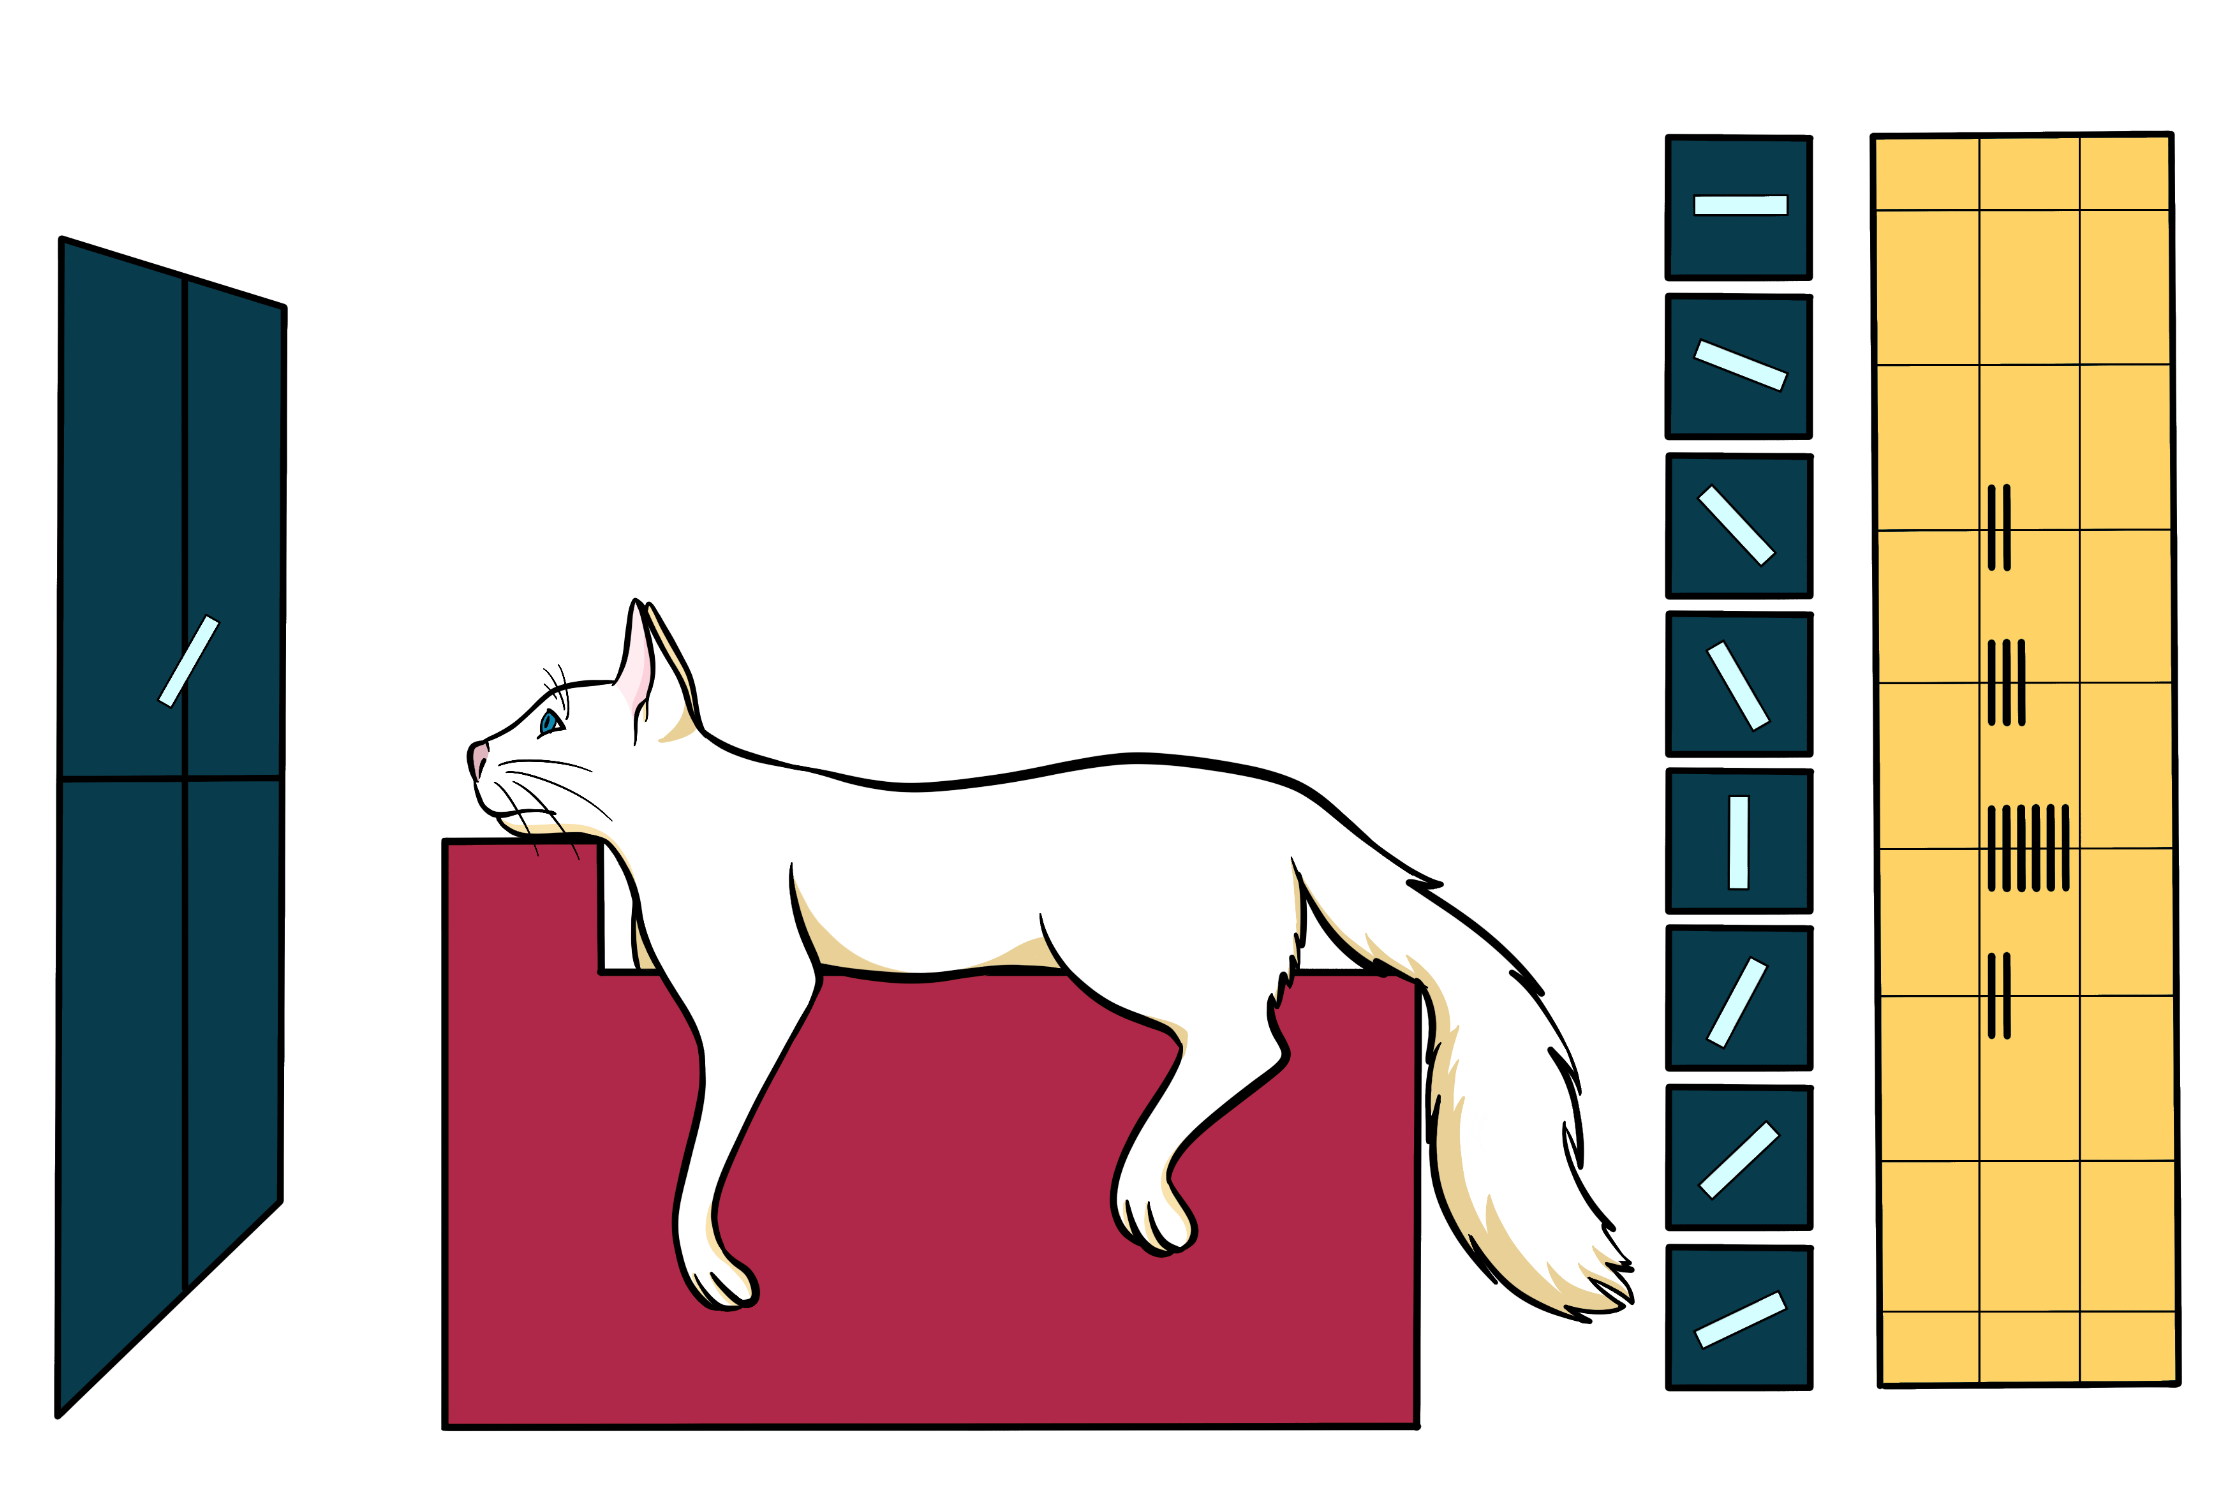
\includegraphics[scale=.3]{figures/cat_experiment.png}
    \caption{Simplified representation of Hubel and Wiesel’s findings on the visual cortex of cats.~\cite{futurelearn2023} }
    \label{fig:lenet}
\end{figure}

\subsection{Image Classification}

At its core, Image Classification is one of the fundamental tasks in computer vision. It involves assigning a predefined label to an input image, usually based on its primary content. For instance, an image containing predominantly a dog would be labeled "dog", irrespective of the breed or its position in the image. In mathematical terms, given an image \(I\), a classifier function \(f\) assigns it a label \(l\) from a set of predetermined labels \(L\):

\[ l = f(I) \]
where \( l \in L \).\\

\begin{figure}[htbp]
    \centering
    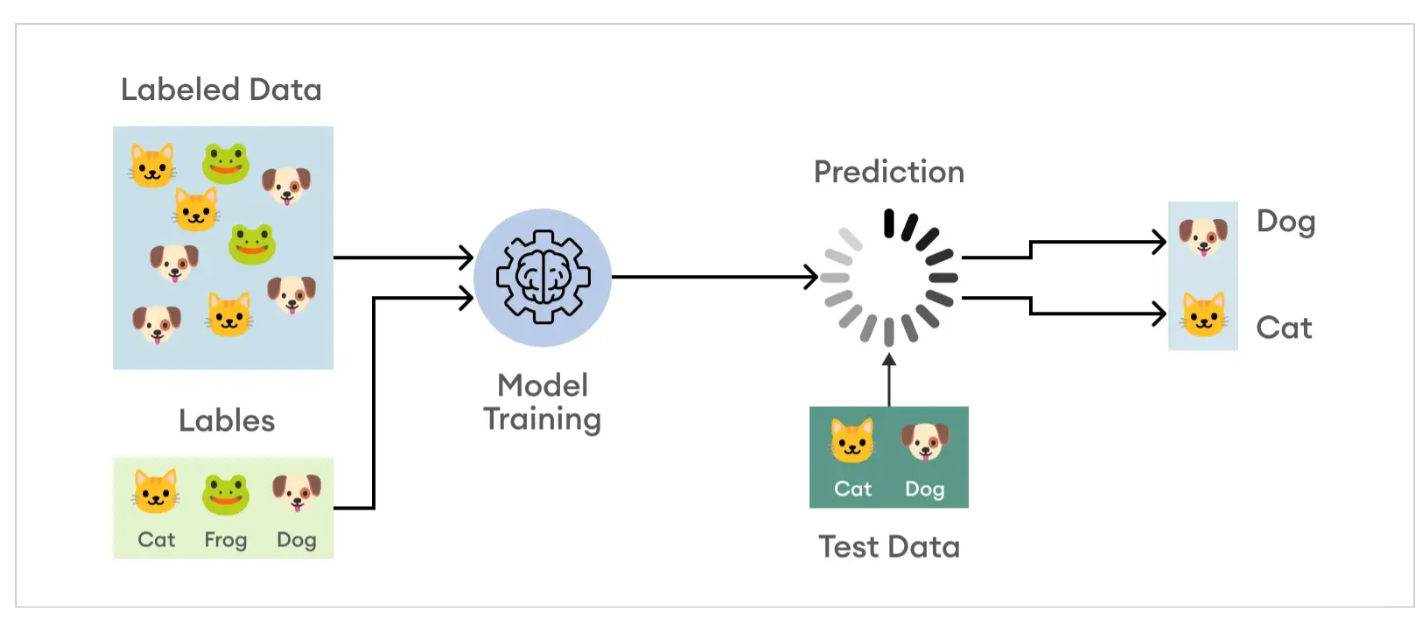
\includegraphics[scale=.5]{figures/image_classification.png}
    \caption{Simple illustration of image classification.~\cite{superannotate2023}}
    \label{fig:lenet}
\end{figure}

\textbf{Applications of Image Classification:}
While the rudimentary idea behind image classification might seem simple, its applications have profound impacts on various sectors:

\begin{itemize}
    \item \textit{Medical Imaging:} Diagnosing diseases by classifying medical images into categories like 'tumor' or 'no tumor'.
    \item \textit{Structural Health Monitoring:} Detecting defects or damages in structures like bridges, buildings, and dams by processing and analyzing images or videos. 
    \item \textit{Agriculture:} Identifying unhealthy plants or predicting the type of crops in satellite imagery.
    \item \textit{Security:} Automated surveillance systems detecting unauthorized or suspicious individuals.
    \item \textit{Retail:} Assisting in automated checkout processes by identifying products.
    \item \textit{Automotive:} In autonomous driving, classifying objects helps vehicles make informed decisions, e.g., distinguishing between pedestrians and lampposts.
    \item \textit{Smart Cities:} Analyzing satellite or drone imagery to plan urban development, detect changes in land use, or estimate population densities.
    \item \textit{Finance:} Document classification to identify types of financial statements or bills.
    \item \textit{Social Media:} Content recommendation based on user's photo uploads or identifying inappropriate content.
\end{itemize}

\textbf{Challenges in Image Classification:}

Despite advances, several challenges remain in image classification:

\begin{itemize}
    \item \textit{Intra-class Variation:} Objects of the same class can appear different under varying lighting, angles, or occlusions.
    \item \textit{Scalability:} As the number of categories increases, distinguishing between them becomes harder.
    \item \textit{Data Imbalance:} Some classes might have fewer training samples than others, leading to biased predictions.
    \item \textit{Transferability:} A model trained on one dataset might not perform well on another due to domain shifts.
\end{itemize}


\section{Reproducibility in Scientific Research}

Reproducibility stands as the foundational pillar upon which the foundation of the scientific method has been built. It functions as a strict check, ensuring that scientific findings remain steady and consistent, regardless of who conducts the experiment.\\

In research, methodological variability often appears as a major challenge. The slightest changes in methodology or experimental procedure can significantly change outcomes. For instance, an experiment conducted at a slightly different temperature or using a slightly different concentration of a reagent can produce different results. As we delve further into research, especially in areas overflowing with big data and high-throughput technologies, the challenges increase. Managing and processing such large amounts of data to ensure reproducibility is a challenging task.\\

Today's research isn't just about test tubes and microscopes; it's closely tied with software. However, as software changes and updates, it introduces another source of inconsistency. An older experiment rerun on a newer software version might yield different results, making reproducibility unclear. This reliance on software, along with the bias towards publishing positive or novel results, means that a significant portion of research, especially those with negative results, remains unpublished.\\

Furthermore, the complexity of the reproducibility issue is highlighted by a survey conducted by Nature, where more than 70\% of the surveyed researchers admitted to having faced challenges in reproducing another scientist's experiments, and over half encountered difficulties reproducing their own experiments. Despite this, most still trust the published literature, showing mixed feelings about reproducibility in the scientific community~\cite{PMID:27225100}.\\

However, the consequences of irreproducible research extend beyond the academic world. The impact of irreproducible research is felt throughout society, leading to wasted resources as other researchers unknowingly follow paths based on incorrect findings. Even more serious, in fields like medicine, the risks are high. Irreproducible research can lead to misguided clinical practices, resulting in wrong treatment methods that can harm patients.\\

\subsection{Irreproducibility in Deep Learning}

Deep within the neural networks of deep learning lies an inherent stochastic nature that brings with it both challenges and opportunities. This randomness, while fundamental to the training processes of deep learning, also introduces a level of unpredictability that can be both a boon and a bane.\\

At the heart of this randomness is the initialization of weights in neural networks. Starting a model's training journey, these weights are often set to random values, acting as the initial step in a long journey towards optimization. Yet, like setting out on a hike from different starting points, these varied initializations can lead the model to different local optima, influencing the final model's performance.\\

Data augmentation, a technique employed to artificially expand training datasets, further introduces variability. By applying transformations like random cropping or rotation, each epoch of training might expose the model to subtle variations of the same data. While this enhances model robustness, it's another source of randomness.\\

Yet, the landscape of randomness in deep learning isn't just about data and weights. Algorithms like Stochastic Gradient Descent (SGD) introduce their own flavor of unpredictability. By using a random subset of data for weight updates, SGD ensures that the model doesn't just memorize data but learns the underlying patterns. However, this very strength is also a source of variability.\\

Beyond these, computational intricacies, such as floating-point precision in digital computations, especially on GPUs, add their own minute variations. Over millions of operations, these tiny discrepancies accumulate, causing significant variability in outcomes.\\

The randomness issue in deep learning is being actively researched. 
Several studies have approached the issue from various angles. 
For instance, Gundersen et al.~\cite{gundersen2022sources}, identified the sources of irreproducibility. 
They found that non-technical sources, such as the initial conditions and the environment of the experiments, affect reproducibility. 
These causes are often related to the mindset and the thinking of the researchers as well as financial constraints. Fig \ref{fig:sources} shows
the non-technical factors that make harder to reproduce any scientific results. These factors indeed valid for deep learning tasks.
Detailed \emph{documentation} with instructions to reproduce to results will help with the reproducibility
and \emph{transparency} on this process would certainly contribute to this cause. Lastly, some \emph{ethics and privacy} regulations could also prevent researchers
to reveal sensitive information, especially in medical domain.
\\

We examine the randomness in this master thesis, which is a technical factor. There are implementation factors and algorithmic factors. These are generally
related with the tooling and the methodology of the experiments. These factors introduce randomness on different level of deep learning process
as a result, variance in the performance occurs. According to Pham et al.~\cite{pham2020problems}, accuracy of the models varies up to \emph{10.8\%}. They conducted a survey as well and
find out that \emph{83.8\%} of the participants unaware of or unsure about implementation level variance. 
Thus, it is reasonable to approach implementation level randomness interrogatively and investigate some standard processes in DL. 
\begin{figure}[htbp]
    \centerline{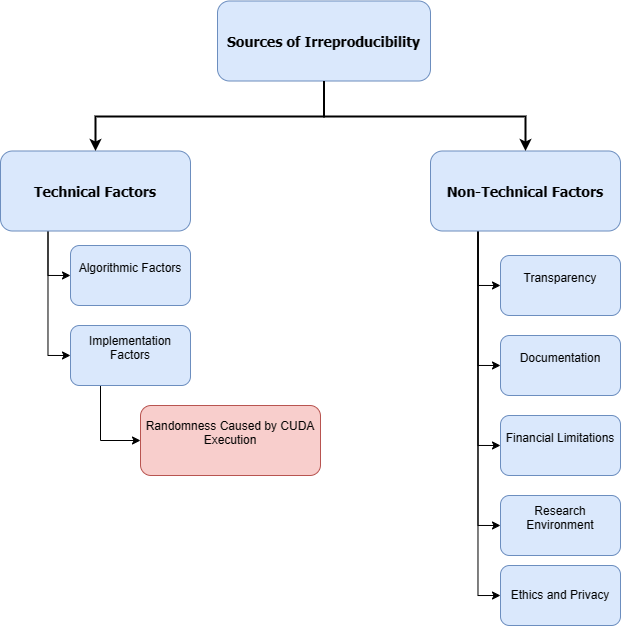
\includegraphics[scale=.5]{figures/Sources.png}}
    \caption{Investigation area of the study.}
    \label{fig:sources}
    \end{figure}
\\
\\
The ripples of this randomness in deep learning extend far and wide. As AI systems become ever more pervasive, from diagnosing diseases to driving cars, unpredictability can pose substantial challenges. Models that yield varying results across runs can complicate evaluations, making direct comparisons challenging. In high-stakes scenarios, like medical diagnoses, this unpredictability can have dire ramifications. Hence, while randomness is an intrinsic aspect of deep learning, understanding, managing, and sometimes mitigating it becomes paramount to harness the true potential of AI.\\
\\

\subsection{Sources of Randomness}
Table \ref{tab:randomness_factors} presents a full list of algorithmic and implementation factors that introduces randomness~\cite{pham2020problems}~\cite{gundersen2022sources}~\cite{zhuang2022randomness}:

\begin{table}[h]
    \centering
    \renewcommand{\arraystretch}{1.5} % Increase row height
    \setlength\tabcolsep{10pt} % Increase space between columns
    \begin{tabular}{|m{0.45\textwidth}|m{0.45\textwidth}|}
    \hline
    \rowcolor{lightgray}
    \textbf{Algorithmic Factors} & \textbf{Implementation Factors} \\
    \hline
    Nondeterministic DL layers that introduce stochasticity & Used framework \\
    \hline
    Random initialization of the weights & Used framework version \\
    \hline
    Hyperparameter optimization & Nondeterministic floating point arithmetic \\
    \hline
    Data augmentation & Parallel execution \\
    \hline
    Data shuffling and ordering & Auto selection of primitive operations \\
    \hline
    Batch ordering & Unpredictability of processing unit \\
    \hline
    \end{tabular}
    \caption{Algorithmic and Implementation Randomness Factors in Deep Learning.}
    \label{tab:randomness_factors}
\end{table}

\subsection{Floating-Point Arithmetics and Parallel Execution}

In the high-performance computing, GPUs have emerged as game-changers. With their vast array of parallel processing units, they have brought unprecedented computational capabilities to the fingertips of developers. NVIDIA's CUDA platform harnesses this power, providing a framework for parallel computing on CUDA-capable GPUs \cite{chetlur2014cudnn}. At the heart of this acceleration lies the intricate dance between floating-point arithmetic and parallel execution.\\

\subsubsection*{Floating-Point Arithmetic: A Double-Edged Sword}

Floating-point arithmetic provides a method to represent and perform operations on real numbers using a finite number of bits. This mathematical framework is fundamental for a multitude of scientific calculations, including those prevalent in deep learning (DL) networks. The primary challenge is that the finite precision of floating-point arithmetic can lead to errors. Although these errors are generally minuscule, their effects can accumulate, notably in iterative algorithms.\\

The IEEE 754 standard delineates the specifics of floating-point arithmetic, fostering consistency across various platforms. This consistency is indispensable, especially given the increasing use of computational methods in scientific research. However, one limitation of the IEEE 754 standard is that, while it prescribes the precision and behavior of singular operations, it doesn't fully govern the sequence of operations or their compound effects. This issue becomes particularly pronounced in parallel computing environments. Here, operations can run concurrently or in an unpredictable sequence, leading to the propagation and magnification of these inherent errors, sometimes resulting in non-deterministic outcomes.

\paragraph{Understanding the Limitations:}

\begin{enumerate}
    \item \textit{Representation Limits:} Not all real numbers can be precisely represented due to the fixed number of bits allocated for floating-point numbers. For instance, the fraction \( \frac{1}{3} \) is a recurring decimal, and its binary representation is similarly recurring. As a result, it's truncated, introducing an error.\\
    
    \item \textit{Rounding Errors:} Numbers that can't be accurately represented lead to rounding errors during operations. For a practical demonstration, in an ideal scenario, \( 0.1 + 0.2 = 0.3 \). Yet, in floating-point arithmetic, this sum might manifest as \( 0.30000000000000004 \) due to inherent representation errors.\\
    
    \item \textit{Error Accumulation:} The cumulative effect of small errors can be significant in iterative processes. Consider an algorithm that repeatedly adds a minuscule value. If the algorithm adds \( 0.0000001 \) a million times, the expected result is \( 0.1 \). However, in floating-point arithmetic, the final sum might diverge slightly from this value.\\
    
    \item \textit{Catastrophic Cancellation:} Subtraction between nearly equivalent floating-point numbers can obliterate significant digits. As an illustrative example, for numbers \( a = 1.0000001 \) and \( b = 1.0000002 \), the difference \( b - a \) should be \( 0.0000001 \). If the precision limits of the system coerce both numbers to round to \( 1.000000 \), the resultant difference becomes zero—a stark contrast to the true value.
\end{enumerate}

In summary, while floating-point arithmetic is a cornerstone of computational methodologies, particularly in DL, its limitations necessitate meticulousness and often compensatory strategies in algorithm design and execution.
\subsubsection*{Parallel Execution in CUDA}

CUDA's parallel execution model divides tasks into threads that are executed across the multiple cores of a GPU. These threads are grouped into blocks, and these blocks are, in turn, organized into grids \cite{chetlur2014cudnn}. This hierarchy allows CUDA to scale computations across different GPU architectures effectively. The figure below illustrates this structure:\\

\begin{figure}[htbp]
\centerline{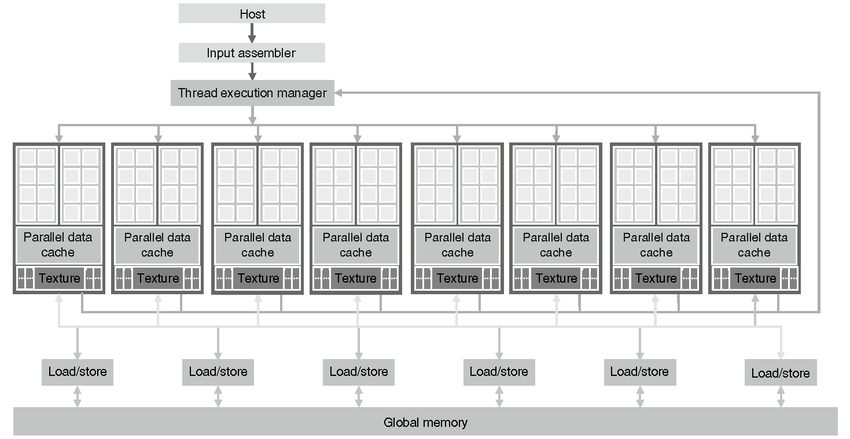
\includegraphics[scale=.5]{figures/cuda.png}}
\caption{CUDA compatible GPU (graphic processor unit) architecture.~\cite{cuda2023} }
\label{fig:cuda}
\end{figure}

However, the inherent nature of parallel execution introduces randomness due to the unpredictable order in which threads are completed. This randomness is exacerbated when combined with the nuances of floating-point arithmetic. Two runs of the same parallel operation can produce slightly different results due to the varying order of execution and the consequent accumulation of floating-point errors.

\subsubsection*{cuDNN: Leveraging CUDA and Introducing Nondeterminism}

cuDNN is a deep neural network GPU-accelerated library that builds upon CUDA \cite{chetlur2014cudnn}. While it greatly boosts the efficiency of DL networks, some of its operations, such as the CUDA convolution benchmarking, are nondeterministic. This nondeterminism stems from both the scheduling of parallel tasks and the intricacies of floating-point precision. Deterministic execution schemes have been proposed to counteract this issue \cite{chou2020deterministic}. However, these schemes can potentially introduce computational overhead.

\subsubsection*{The Trade-Off: Performance vs. Reproducibility}

There's a delicate balance between performance and reproducibility in parallel computing. Deterministic execution schemes increase the reproducibility and credibility of DL networks, making results more trustworthy and comparable across runs. However, they may come at the cost of increased computational time, which could be a significant drawback in time-sensitive applications or large-scale computations. It is, therefore, essential to analyze and understand these trade-offs carefully, tailoring solutions to specific use-cases and experimental setups.\\

In conclusion, the interplay between floating-point arithmetic and parallel execution in CUDA is a complex one. While it offers immense computational power, it also brings forth challenges in reproducibility. As researchers and developers, it's our responsibility to approach these challenges head-on, understanding their roots and implications, and crafting solutions that balance both performance and reproducibility.

\section{Frameworks and Tools}
The success and efficiency of any scientific study often hinge on the careful selection and proficient use of the right computational tools and frameworks. In the scope of this study, several tools and frameworks have been adopted, each with its unique benefits and contributions to the overall experiment. Here, we provide a brief overview of these tools and their significance in the research.

\begin{table}[h]
    \centering
    \renewcommand{\arraystretch}{1.5}
    \begin{tabular}{|l|p{10cm}|}
    \hline
    \textbf{Framework/Tool} & \textbf{PyTorch} \\
    \hline
    \textbf{Publisher} & Facebook's AI Research lab (FAIR) \\
    \hline
    \textbf{Overview} & An open-source deep learning framework with a dynamic computational graph, PyTorch is versatile and suited for research. It allows on-the-fly graph modifications. \\
    \hline
    \textbf{Role in the Experiment} & PyTorch was central to our study, aiding in the design, training, and evaluation of deep learning models. Its adaptability supported quick prototyping and its extensive library eased the deployment of various architectures and methodologies. \\
    \hline
    \end{tabular}
    \caption{Overview of PyTorch}
\end{table}

\begin{table}[h]
    \centering
    \renewcommand{\arraystretch}{1.5}
    \begin{tabular}{|l|p{10cm}|}
    \hline
    \textbf{Framework/Tool} & \textbf{Weights and Biases (W\&B)} \\
    \hline
    \textbf{Publisher} & Weights \& Biases, Inc. \\
    \hline
    \textbf{Overview} & W\&B is crafted to assist researchers in tracking and visualizing ML experiments. It encapsulates features like hyperparameter tuning, model visualization, and performance tracking. \\
    \hline
    \textbf{Role in the Experiment} & W\&B was integral for experiment management, used for logging results, visualizing model dynamics, and comparing architectures and hyperparameters. \\
    \hline
    \end{tabular}
    \caption{Overview of Weights and Biases}
\end{table}

\begin{table}[h]
    \centering
    \renewcommand{\arraystretch}{1.5}
    \begin{tabular}{|l|p{10cm}|}
    \hline
    \textbf{Framework/Tool} & \textbf{SLURM} \\
    \hline
    \textbf{Publisher} & SchedMD \\
    \hline
    \textbf{Overview} & SLURM is an open-source job scheduler, pivotal for resource allocation in multi-user clusters. It's a mainstay in high-performance computing due to its scalability. \\
    \hline
    \textbf{Role in the Experiment} & Given the computational demands of deep learning, SLURM managed our job submissions. It optimized resource allocation, enabling parallel experiment execution without contention. \\
    \hline
    \end{tabular}
    \caption{Overview of SLURM}
\end{table}

The synergy of these tools and frameworks enabled a seamless, efficient, and insightful experimental process. PyTorch offered the foundational deep learning capabilities; Weights and Biases ensured that experiments were tracked, visualized, and optimized; and SLURM managed the computational resources effectively. Together, they ensured that the research was conducted in a structured, efficient, and reproducible manner.
 
\section{Mathematical Evaluation}

In the thesis, several mathematical tools and methods are used to evaluate the results. In this section, we explain these tools and methods.

\subsection*{Standard Variance}
Standard Variance, denoted as \( \sigma^2 \), is calculated using the formula:
\[ \sigma^2 = \frac{1}{n-1} \sum_{i=1}^n (x_i - \bar{x})^2 \]
where:
\begin{itemize}
    \item \( n \) is the number of observations,
    \item \( x_i \) is each individual observation,
    \item \( \bar{x} \) is the mean of all observations.
\end{itemize}
Standard Variance is crucial in machine learning and statistics to understand the dispersion and to normalize the data. It's also vital for gauging the accuracy and the reproducibility of models by analyzing the variance in predictions.

\subsection*{Cosine Similarity}
Cosine Similarity is a metric used to measure how similar two vectors are, regardless of their size. The formula for cosine similarity \( S_C \) between two vectors \( A \) and \( B \) is given as:
\[ S_C(A,B) = \frac{{\mathbf{A} \cdot \mathbf{B}}}{{\|\mathbf{A}\|\|\mathbf{B}\|}} = \frac{{\sum_{i=1}^{n}{A_iB_i}}}{{\sqrt{\sum_{i=1}^{n}{A_i^2}}\sqrt{\sum_{i=1}^{n}{B_i^2}}}} \]
where \( n \) is the dimension of the vectors.
Cosine similarity is extensively used in machine learning for understanding the similarity between vectors or entities, which is fundamental in algorithms like nearest neighbors, clustering, and also in recommendation systems.

\subsection*{T-Test with Population Mean}
The One Sample T-Test is a statistical method used to determine whether the mean of a single sample is significantly different from a known or hypothesized population mean. The formula for the one-sample t-test is given by:
\[ t = \frac{( \bar{x} – \mu)}{(s / \sqrt{n})} \]
where:
\begin{itemize}
    \item \( \bar{x} \) is the sample mean,
    \item \( \mu \) is the theoretical population mean,
    \item \( s \) is the sample standard deviation,
    \item \( n \) is the sample size.
\end{itemize}
The population mean can also be estimated as:
\[ \text{Population mean} = \text{Sample mean} + T \times (\text{Standard error of the mean}) \]

\subsection*{Kruskal-Wallis Test}
The Kruskal-Wallis test is a non-parametric method for testing whether samples originate from the same distribution. It is used for comparing more than two samples that are independent, or not related. The formula for the Kruskal-Wallis test is:
\[ H = \left(N-1\right)\frac{\sum_{i=1}^g n_i(\bar{r}_{i\cdot} - \bar{r})^2}{\sum_{i=1}^g\sum_{j=1}^{n_i}(r_{ij} - \bar{r})^2} \]
where:
\begin{itemize}
    \item \( N \) is the total number of observations across all groups,
    \item \( g \) is the number of groups,
    \item \( n_{i} \) is the number of observations in group \( i \),
    \item \( \bar{r}_{i\cdot} \) is the average rank of group \( i \),
    \item \( \bar{r} \) is the average rank of all the data,
    \item \( r_{ij} \) is the rank of observation \( j \) in group \( i \).
\end{itemize}

\subsection*{ANOVA Test}
Analysis of Variance (ANOVA) is a statistical method used to test differences between two or more means. It divides the variance in a dataset into component parts associated with different sources of variation. In its simplest form (One-Way ANOVA), it can be used to compare the means of three or more independent groups. ANOVA partitions the total sum of squares into components related to the effects used in the model, as expressed in:
\[ SS_{\text{Total}}=SS_{\text{Error}}+SS_{\text{Treatments}} \]
The F-test statistic in ANOVA is calculated as:
\[ F = \frac{MS_{\text{Treatments}}}{MS_{\text{Error}}} = \frac{SS_{\text{Treatments}}/(I-1)}{SS_{\text{Error}}/(n_{T}-I)} \]
where:
\begin{itemize}
    \item \( MS \) is the mean square,
    \item \( I \) is the number of treatments,
    \item \( n_T \) is the total number of cases.
\end{itemize}
